\section{Карта заменяемости и априорный критерий}\label{sec:criterion}

Кривые «первые $k$ слоёв» отвечают на вопрос о префиксе модели, но не
говорят, какие слои заменяемы вообще и можно ли это предсказать без
запуска замены. Для этого мы заменяем \emph{по одному} слою
$\ell = 0,\dots,27$ при неизменных остальных: внимание "--- окном 64 со
стоком, MLP "--- отбором 25\,\% нейронов по готовым активациям; для
сравнения на вход слоя $\ell$ подаётся гауссово возмущение с
относительной нормой 2\,\%. Качество "--- KL к исходной модели на 8 окнах
по 1024 токена. Параллельно на состояниях учителя считаются статистики,
не требующие замены: масса внимания вне окна (без стока), локальная
ошибка окна на выходе блока внимания, доля вклада 25\,\% сильнейших
нейронов в выход MLP и локальная ошибка их отбора.

\begin{figure}[t]
\centering
\figorpending{figures/map.pdf}{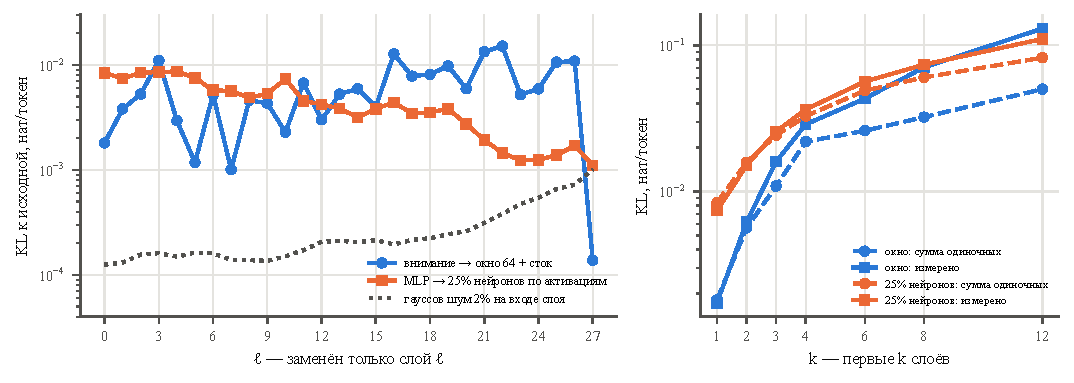
\includegraphics[width=\linewidth]{figures/map.pdf}}
\caption{Слева "--- карта заменяемости Qwen3-0.6B: KL при замене только
слоя $\ell$ (внимание "--- окно 64 + сток; MLP "--- 25\,\% нейронов) и при
изотропном шуме 2\,\% на его входе. Справа "--- аддитивность: сумма KL
одиночных замен первых $k$ слоёв против измеренного KL при их
одновременной замене.}
\label{fig:map}
\end{figure}

\begin{table}[t]
\centering
\small
\IfFileExists{tables/criterion.tex}{\begin{tabular}{llc}
\toprule
Блок & Статистика (без запуска замены) & Спирмен с KL \\
\midrule
Внимание & масса внимания вне окна & 0.37 \\
 & локальная ошибка окна (отн. выхода внимания) & 0.82 \\
 & ошибка относительно остаточного потока & 0.52 \\
 & то же $\times$ чувствительность слоя & 0.77 \\
MLP & $1-$ доля вклада 25\% сильнейших нейронов & 0.92 \\
 & локальная ошибка отбора (отн. выхода MLP) & 0.82 \\
 & ошибка относительно остаточного потока & 0.97 \\
 & то же $\times$ чувствительность слоя & 0.96 \\
\bottomrule
\end{tabular}
}{\textcolor{red}{[ожидает прогона]}}
\caption{Ранговая корреляция Спирмена (28 слоёв) между статистиками
слоя, вычисленными без замены, и KL при его одиночной замене.}
\label{tab:criterion}
\end{table}

\paragraph{Карта по глубине.} Для внимания KL одиночной замены меняется
на два порядка по глубине и немонотонно: легче всего заменяются слои
27, 7, 5, 0, 10 и 4 ($\mathrm{KL} \le 0.003$), труднее всего "--- 22, 21
и 16 ($\ge 0.013$); слой-сток 3 оказывается одним из трудных (0.011),
так как помимо стока содержит головы с дальним контекстом. Для MLP
картина противоположна исходной посылке о «простых первых слоях»:
KL максимален в слоях 0--4 (0.0084--0.0087) и минимален в слоях 21--27
(0.0011--0.0019). Иными словами, MLP первых слоёв "--- самые
\emph{незаменяемые} отбором нейронов во всей модели, а поздних "--- самые
заменяемые; это согласуется с ростом разреженности активаций по глубине
и с ролью ранних MLP как «детокенизатора»~\cite{elhage2021framework}.

\paragraph{Априорный критерий.} Для MLP достаточно одной статистики: доля
вклада 25\,\% сильнейших нейронов предсказывает KL одиночной замены с
корреляцией 0.92, а локальная ошибка отбора, отнесённая к норме
остаточного потока, "--- 0.97 (табл.~\ref{tab:criterion}). Для внимания
масса вне окна предсказывает плохо (0.37): важно не то, сколько массы
теряется, а как меняется выход блока; локальная ошибка окна даёт 0.82.

\paragraph{Воспроизводимость на 1.7B.} Все три наблюдения повторяются
на Qwen3-1.7B без подгонки: корреляции Спирмена составляют 0.91--0.96 для
MLP и 0.33--0.77 для внимания; карта по глубине почти та же (внимание
легче всего заменяется в слоях 27, 5, 7, 10, 0, труднее всего "--- в 21,
22 и слое-стоке 3; MLP слоёв 21--27 заменяется в 15--20 раз легче, чем
слоёв 3--5); сумма одиночных KL совпадает с измеренной для отбора
нейронов (0.043 против 0.050 при $k=8$) и занижает её для окна (0.035
против 0.066).

\paragraph{Аддитивность и направление ошибки.} Для отбора нейронов сумма
KL одиночных замен первых $k$ слоёв почти совпадает с измеренным KL при
их совместной замене (0.024 против 0.026 при $k=3$, 0.082 против 0.111
при $k=12$). Для окна сумма занижает: 0.011 против 0.016 при $k=3$ и
0.050 против 0.130 при $k=12$, то есть ошибки окна взаимодействуют и
накапливаются суперaддитивно. Та же разница видна по отношению KL к
энергии возмущения: ошибка окна вредит в 2--6 раз сильнее изотропного
шума той же энергии на том же слое, а ошибка отбора нейронов ведёт себя
как шум (отношение 0.9--1.6). Прямое измерение структуры ошибок
подтверждает это: ковариация ошибки на выходе модели при замене окном
имеет эффективный ранг 19--115 (на 8 главных компонент приходится
20--44\,\% энергии), при отборе нейронов "--- 83--277 (11--23\,\%); средний
косинус между ошибками от замен разных слоёв равен 0.071 для окна против
0.022 для MLP (0.135 против 0.034 среди первых шести слоёв). Ошибки окна
низкоранговы и согласованы между слоями "--- они складываются; ошибки
отбора нейронов близки к изотропному шуму и складываются по энергии.

\paragraph{CATS не работает в ранних слоях.} Пороговый отбор по величине
$|\mathrm{act}(\mathrm{gate})|$~\cite{lee2024cats}, который в литературе
применяют ко всей модели, в одиночной замене слоя проигрывает отбору по
полному вкладу нейрона в 5--37 раз в слоях 0--5 и лишь в 1.3--3 раза в
слоях 22--27 (рис.~\ref{fig:cats}); на 1.7B "--- в 2.5--5.6 и 1.3--3 раза.
При замене первых трёх слоёв CATS с 25\,\% активных нейронов даёт
$+70\,\%$ PPL, при $k=4$ "--- почти $+300\,\%$. В ранних слоях важен
критерий отбора, и именно там дешёвые пороговые методы не применимы.

\begin{figure}[t]
\centering
\figorpending{figures/cats_depth.pdf}{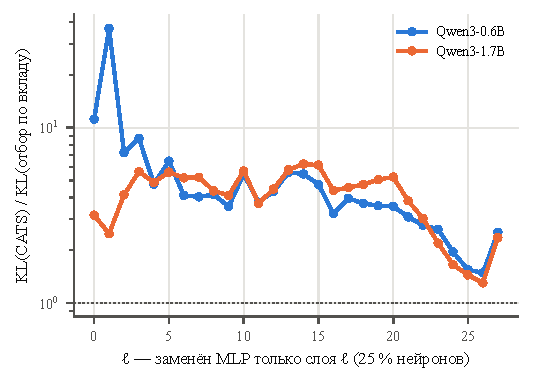
\includegraphics[width=0.5\linewidth]{figures/cats_depth.pdf}}
\caption{Отношение KL при пороговом отборе CATS к KL при отборе 25\,\%
нейронов по вкладу, замена MLP одного слоя $\ell$.}
\label{fig:cats}
\end{figure}

\paragraph{Почему MLP ранних слоёв незаменим.} Карта фиксирует факт, а
не причину. Мы сопоставили KL одиночной замены MLP с пятью свойствами
слоя, измеренными на состояниях учителя (Qwen3-0.6B). Сильнее всего с KL
связана концентрация вклада (доля 25\,\% сильнейших нейронов, Спирмен
$-0.92$) и число существенно активных нейронов (вклад выше $1\,\%$ от
максимального по токену, Спирмен $+0.70$): в слоях 0--5 активны
$1\,900$--$2\,300$ нейронов из $3\,072$, в слоях 21--26 "--- $1\,200$--$1\,400$,
в слое 27 "--- 275. Второй фактор "--- величина записи: норма выхода MLP
относительно остаточного потока равна $0.45$--$0.72$ в слоях 0--4 и
$0.22$--$0.40$ в слоях 11--26 (Спирмен $+0.44$); эффективный ранг выхода
ведёт себя так же ($+0.52$). Гипотеза о том, что ранние MLP пишут именно
в подпространство, которое читают ключи и запросы слоя-стока, не
подтвердилась: доля их выхода в этом подпространстве ($0.74$) совпадает
со случайным подпространством той же размерности ($0.78$). Наконец,
ошибка отбора на продолжениях слов выше, чем на началах, только в слоях
0--5 ($0.18$--$0.22$ против $0.14$--$0.19$), а с седьмого слоя разницы нет.
Итог: MLP ранних слоёв пишет в остаточный поток большие, плотные и
высокоранговые векторы "--- в особенности когда собирает слово из
нескольких токенов, "--- и любое подмножество нейронов теряет заметную долю
такого вектора; MLP поздних слоёв разрежен и мал относительно уже
большого остаточного потока, поэтому его легко заменить.
На Qwen3-1.7B все три зависимости повторяются (ранговая корреляция концентрации
вклада с KL замены $-0.91$, доли активных нейронов $+0.75$); на SmolLM2 они
слабеют "--- см. абзац <<Второе семейство>> ниже.

\paragraph{Что не покрывается словарём.} Разбиение ошибки остаточного
потока на входе слоя~3 по типам токенов показывает, чего не хватает
каждой замене. Табличная замена MLP по токену (M-O2, робастная; средняя
относительная ошибка 0.31) хуже всего на продолжениях слов (0.59 против
0.25--0.30 для пунктуации, начал слов и цифр), и десять худших токенов "---
это фрагменты вроде <<se>>, <<ga>>, <<ter>>, <<ly>>: сборка слова из
кусков требует контекста соседей, которого у таблицы нет. У предиктора
нейронов M-O4 (0.21) тот же профиль в смягчённом виде (0.41 на
продолжениях). Окно (0.11), напротив, одинаково хорошо справляется с
началами и продолжениями слов (0.09--0.10), а хуже всего "--- на переводах
строки и разделителях (0.17--0.27): редкие структурные токены, которым
нужен далёкий контекст. Иными словами, первые слои делают две разные
вещи: локальную сборку слов из кусков, которую окно сохраняет, а словарь
теряет, и разметку структуры документа, для которой нужен хвост
контекста.

\subsection{Планировщик замен по априорным статистикам}

Критерий позволяет выбирать, \emph{что} заменять, не запуская замены.
Мы подгоняем на Qwen3-0.6B две лог-линейные зависимости KL одиночной
замены от статистик (локальная ошибка окна для внимания; ошибка отбора
относительно остаточного потока для MLP) и показатель суперaддитивности
внимания $\gamma=0.47$ по кривой howmany, затем применяем их к
Qwen3-1.7B \emph{по её собственным статистикам}: предсказанные KL
одиночных замен коррелируют с измеренными на уровне 0.75 (внимание) и
0.94 (MLP). Жадный план из $m$ компонент с минимальным предсказанным
итогом сравнивается с двумя префиксами: первые $m/2$ слоёв целиком и
окно в первых $m$ слоях (рис.~\ref{fig:planner}). При $m=6$ план даёт
KL $0.0031$ ($+0.1\,\%$ PPL) против $0.0335$ ($+3.2\,\%$) и $0.0453$
($+4.0\,\%$); при $m=12$ "--- $0.0070$ ($+0.4\,\%$) против $0.083$ и
$0.114$. План состоит из MLP поздних слоёв (23--27) и внимания слоя~0, то
есть критерий сам уводит замену от префикса в хвост модели. На 0.6B
(подгонка и проверка на одной модели) выигрыш тот же: при $m=12$ "---
$2.2\,\%$ против $9.5$ и $13.9\,\%$.

\begin{figure}[t]
\centering
\figorpending{figures/planner.pdf}{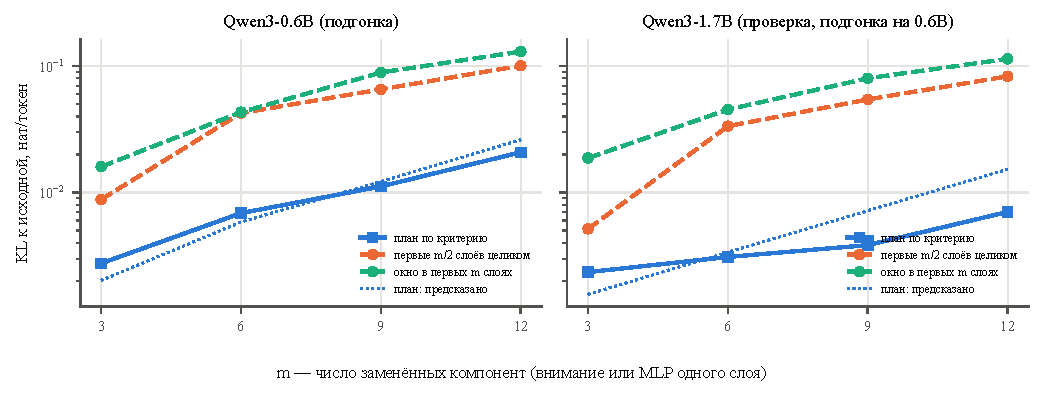
\includegraphics[width=\linewidth]{figures/planner.pdf}}
\caption{Планировщик по априорным статистикам против замены префикса:
KL в зависимости от числа заменённых компонент $m$. Зависимости
подогнаны на Qwen3-0.6B (слева) и без изменений применены к Qwen3-1.7B
(справа); пунктир "--- предсказание плана.}
\label{fig:planner}
\end{figure}

\paragraph{Второе семейство.} Те же зависимости, подогнанные на
Qwen3-0.6B, применены без изменений к SmolLM2-1.7B и Llama-3.2-1B по их
собственным статистикам. Планировщик переносится: на SmolLM2 при $m=6$
план даёт KL 0.026 ($+2.6\,\%$ PPL) против 0.145 ($+15.8\,\%$) у префикса
из трёх блоков и 0.49 ($+62\,\%$) у окна в шести первых слоях (с
позиционным стоком); план состоит из внимания слоёв 0, 22, 23 и MLP
слоёв 20--22, то есть снова уходит из начала модели. На Llama-3.2-1B при
$m=6$ "--- $7.9\,\%$ против 20.7 и 22.3\,\%, при $m=12$ "--- 28.1 против
35.7 и 47.2\,\%; при $m=3$ префикс из блока~0 целиком ($3.2\,\%$) лучше
плана ($4.6\,\%$): у 16-слойной модели предсказание KL внимания
завышено. Критерий для MLP переносится хуже: ранговая корреляция
концентрации вклада с KL замены составляет $-0.25$ на SmolLM2 и $-0.51$
на Llama-3.2-1B против $-0.91$ на Qwen3-1.7B, а поздние MLP у SmolLM2 не
дешевле ранних (KL одиночной замены 0.004--0.0075 по всей глубине, слой~23
"--- самый дорогой), тогда как у Qwen3 они в 5--30 раз дешевле. Сравнение
CATS с отбором по вкладу (отношение ошибок 1.8--3.7 по всем 24 слоям) и
аддитивность воспроизводятся.
